\chapter{TECNOLOGIAS UTILIZADAS} \label{cap:theONE}

É objetivo deste capítulo descrever as tecnologias utilizadas para a elaboração da técnica objetivada neste trabalho.

Inicialmente é apresentado o simulador The ONE, responsável por permitir implementação e teste da técnica elaborada utilizando, para tanto a plataforma Java. Para tanto, as principais características do simulador são abordadas, tendo com foco a descrição da arquitetura modular do simulador.

Após a apresentação do simulador The ONE, a plataforma Java é brevemente abordada e, em seguida, é apresentada a ferramenta Gnuplot, responsável pela geração dos gráficos de apresentação dos resultados obtidos no capítulo \ref{cap:testes}.

Ao final do capítulo, é apresentada a conclusão, onde é realizado fechamento deste capítulo.

\section{Simulador The ONE}\label{sec:theONE}

O \emph{The Opportunistic Network Environment Simulator}, ou apenas The ONE, é uma ferramenta open source modular construída utilizando a plataforma Java e que permite a simulação de DTNs e implementa os principais mecanismos necessários para funcionamento dessas redes, como algoritmos de disseminação e gerenciamento de mensagens \cite{keranen2009one}. A Figura \ref{theONE} apresenta os módulos do simulador e os seus respectivos relacionamentos. 

Quanto a sua utilização, o The ONE baseia-se na definição de um cenário de simulação onde é possível configurar diversos elementos, como eventos, protocolos de encaminhamento, modelos de movimentação, características dos dispositivos e relatórios a serem gerados. Tais itens são melhor detalhados nas subseções a seguir, começando pelo Encaminhamento de Mensagens, passando pelo Módulo de Energia, Modelos de Movimento, Eventos, Relatórios e Automação de Testes, Dispositivos e, finalmente, uma breve apresentação da Interface Gráfica do mesmo.

\begin{figure}[htp!]
    \centering
    \includegraphics[width=1\textwidth]{figuras/cap_3/secao_1/TheONEArchtecture.png}
    \caption{Arquitetura do simulador The ONE \cite{keranen2009one}.}
    \label{theONE}
\end{figure}

\subsection{Encaminhamento de Mensagens}

O simulador The ONE nativamente é compatível com os principais protocolos de encaminhamento existentes em DTNs. Destacando-se os protocolos Prophet, Epidemic Routing, Spray-and-Wait e Direct Contact, que foram explanados na subseção \ref{subsec:encaminhamento_mensagens}. Todos os protocolos são implementados junto ao módulo \emph{routing} exibido na Figura \ref{theONE}.

A arquitetura modular do simulador possibilita grande flexibilidade quando deseja-se testar novos protocolos, bastando para tanto implementar o modelo desejado e integrá-lo ao módulo \emph{routing}. Para isso, o desenvolvedor do novo protocolo a ser testado precisa apenas herdar e sobrescrever, caso necessário, as características da classe \emph{ActiveRouter}, que, por sua vez, define operações básicas comuns de todos os protocolos de encaminhamento voltado para as DTNs, como decisões estratégicas de envio e recepção de mensagens e o gerenciamento do buffer de mensagens.

Quanto à simulação dos protocolos, um dos principais diferenciais do simulador escolhido é a possibilidade de definir grupos de nós, onde, cada grupo, pode executar diferentes protocolos de encaminhamento e possuir detalhes de hardware únicos, como tamanho dos buffers de armazenamento e antenas de rádio com diferentes capacidades.

\subsection{Módulo de Energia}
\label{modulo_energia}
Integrado ao módulo \emph{Routing}, há o módulo \emph{Energy Model}, que é responsável por realizar a simulação das baterias e do seu respectivo consumo. Esse módulo foi implementado por \cite{denis_artigo} e foi integrado oficialmente ao simulador The ONE na sua última versão, a 1.6, lançada em 7 de outubro de 2015 \cite{theOne_github}.

O módulo de energia desenvolvido por \cite{denis_artigo} considera que todos os dispositivos possuem cinco estados básicos de funcionamento:

\begin{itemize}
    \item \textbf{Desligado:} Neste estado, o nó não pode fazer uso de suas interfaces de rede, seja por falta de energia ou por uma decisão feita pelo protocolo de encaminhamento, como por exemplo economizar energia durante algum tempo. Além disso, não é possível estabelecer conexões com outros nós e, como consequência, não pode enviar e receber mensagens;
    \item \textbf{Inativo:} O nó, neste estado, tem as suas interfaces de rede ligadas mas está adormecido. Todavia, pode ser detectado e contatado por outros nós. Numa situação real este estado é responsável pelo consumo muito pequeno de energia, porém ele não é considerado por parte deste módulo;
    \item \textbf{Buscando:} Neste estado o nó encontra-se na procura por nós vizinhos para que possa estabelecer contato e, posteriormente, receber e enviar mensagens. Em suma, os nós entram periodicamente neste estado de acordo com o intervalo de busca pré-definido;
    \item \textbf{Transmitindo:} Estado onde o nó envia mensagens para outro;
    \item \textbf{Recebendo:} Estado onde o nó está recebendo mensagens de outro.
\end{itemize}

De acordo com \cite{denis_artigo}, é a partir do estado que o nó se encontra que o controle do consumo energia é realizado. Quando o nó tem sua interface no estado Inativo não é considerado o consumo de energia. Entretanto, quando o nó encntra-se apto para efetuar operações de busca por outros nós, envio e recebimento de mensagens o consumo é considerado de acordo com as propriedades definidas. Ao realizar uma operação de busca por outros nós, o módulo calcula a quantidade de energia consumida e decrementa da quantidade atual por meio do método \emph{reduceEnergy}. Quando se trata das operações de envio e recepção de mensagens, o módulo opera de forma um pouco diferente, pois decrementa a quantidade de energia definida a cada segundo de duração da operação de envio ou recebimento.

\subsection{Modelos de Movimento}

Os modelos de movimentação são responsáveis por descrever como será o deslocamento dos nós dentro da rede e são suportados diversos deles pelo módulo \emph{Movement Models}. O simulador apresenta nativamente o suporte a dois principais tipos de modelos de movimentação: sintéticos ou capturados de uma DTN real.

Os modelos sintéticos caracterizam-se por gerarem, seja aleatoriamente ou não, o caminho que os nós realizam no ambiente simulado. Podendo, para tanto, serem definidos mapas por onde nós podem se movimentar. Já os modelos capturados, são caracterizados por serem obtidos de uma DTN real e convertidos para o padrão de representação do simulador que, a partir daí, define o padrão de comportamento dos nós como o sendo do ambiente real.

Capturar a movimentação de nós num ambiente real e utilizá-los dentro de um ambiente simulado permite verificar como a rede pode se comportar quando são utilizados protocolos diferentes dos que estão em operação no ambiente real, além, é claro, de permitir maior grau de realismo nas simulações.

\subsection{Eventos}

Os eventos, gerados e processados pelo módulo \emph{Event Generators}, nada mais são que as mensagens trocadas entre nós da rede simulada. As mensagens são sempre "de um para um", ou seja, são originadas em um nó específico e destinadas a outro nó específico.

O simulador permite que sejam configurados parâmetros como o intervalo de tempo que um dispositivo gera mensagens para outro além do tamanho das mesmas. Pode-se, é claro, definir para ambos os parâmetros um valor mínimo e máximo, ficando o simulador responsável por gerar valores aleatórios dentro do intervalo definido.

\subsection{Relatórios e Automação de Testes}

Dentre todas as funcionalidades já apresentadas destaca-se a geração de relatórios pelo módulo \emph{Visualization and Results} e a possibilidade de automatização de testes implementada pelo módulo principal \emph{Simulation Engine}. 

A geração de relatórios têm sua importância destacada diante da necessidade de avaliar o comportamento da rede diante de parâmetros definidos e, muito além disso, testar novas técnicas implementadas dentro do simulador. Existem diversos relatórios disponíveis, destacando-se para utilização neste trabalho os seguintes:

\begin{itemize}
    \item \textbf{MessageDeliveryReport:} Este relatório detalha com alta granularidade a quantidade acumulada de mensagens entregues e geradas, além da probabilidade de entrega de mensagens da rede de acordo com o tempo de simulação;
    \item \textbf{EnergyLevelReport:} Tendo sido desenvolvido por \cite{denis_artigo}, este relatório detalha a quantidade de energia contida nas baterias de cada um dos dispositivos de acordo com o tempo de simulação, possibilitando o cálculo da linha de tendência de consumo e a quantidade média de energia armazenada nas baterias.
\end{itemize}

Quanto a automação dos testes, o simulador permite programação de testes por meio de arquivos de configuração e a sua execução a partir da linha de comando em modo batch. A cada teste realizado o simulador gera os respectivos relatórios de teste para que possam ser analisados a fundo posteriormente.

\subsection{Dispositivos}

O simulador The ONE permite configurar grupos de nós, onde, cada um deles, possui uma determinada quantidade de dispositivos com características específicas, como velocidade de movimentação, modelo de movimento, interfaces de rede e capacidade das baterias. Quanto às interfaces de rede, é possível configurar a distância máxima de alcance do sinal de rádio e a velocidade máxima que ela pode operar.

A possibilidade de criar grupos com diversas características únicas permite verificar a interoperabilidade entre os protocolos de encaminhamento, além de simular o comportamento da rede quanto a existência de nós com características distintas.

\subsection{Interface Gráfica}

O simulador permite a visualização em tempo real da simulação por meio de sua interface gráfica, apresentada na Figura \ref{interface_theONE}.  É possível acompanhar individualmente a movimentação dos nós, o estado (ligado/desligado), alcance das interfaces, situação dos buffers e o estado das conexões (up/down/relay). A Figura \ref{node_theONE} apresenta os detalhes individuais do nó \emph{p28} durante uma simulação realizada utilizando o The ONE.

\begin{figure}[htp!]
    \centering
    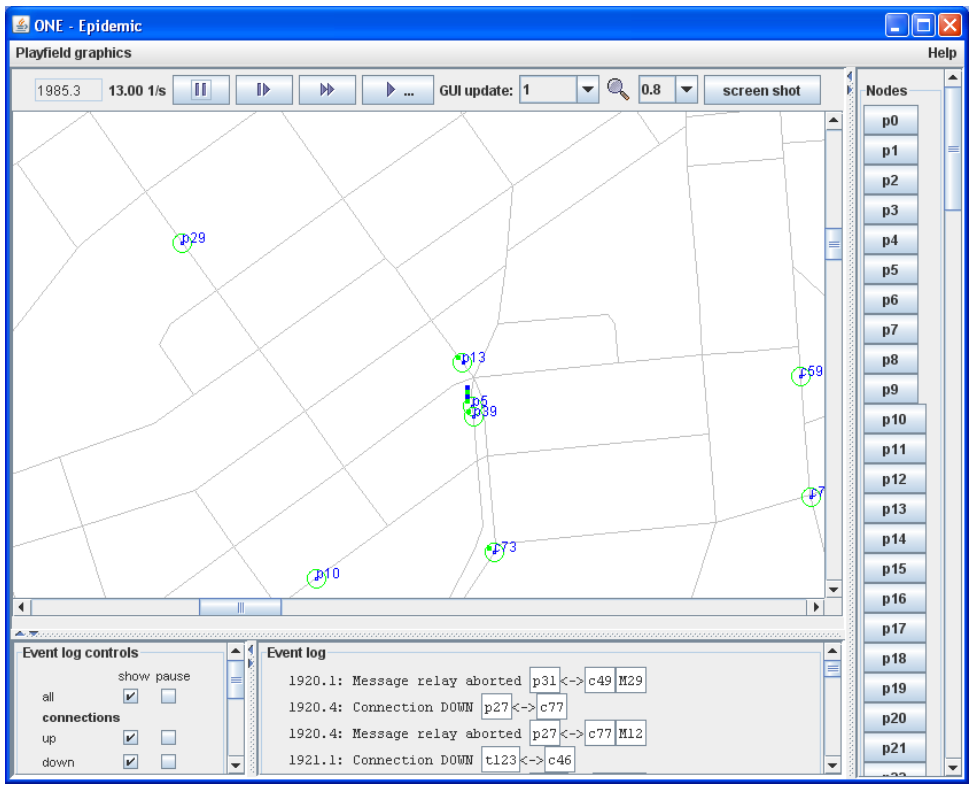
\includegraphics[width=1\textwidth]{figuras/cap_3/secao_1/interface_theONE.PNG}
    \caption{Interface do Simulador The ONE \cite{keranen2009one}.}
    \label{interface_theONE}
\end{figure}

\begin{figure}[htp!]
    \centering
    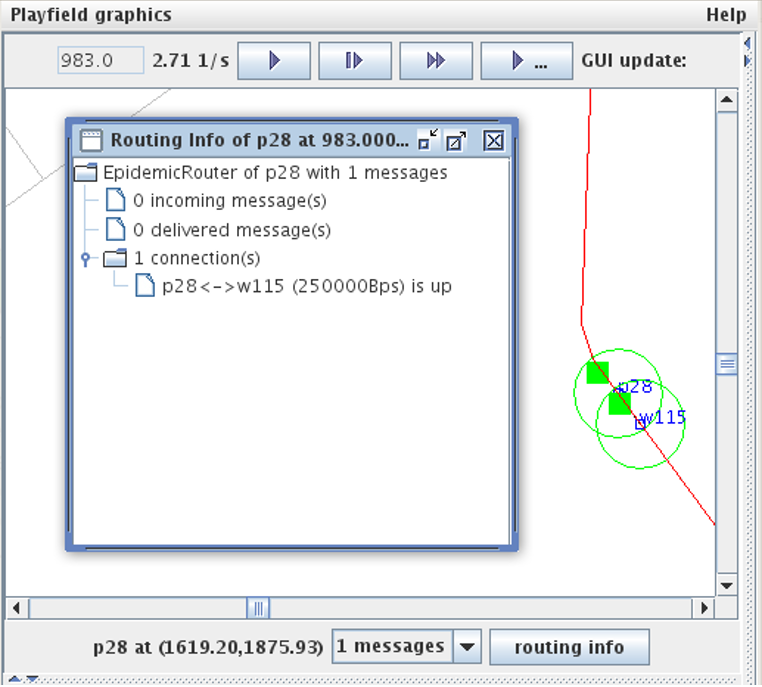
\includegraphics[width=0.6\textwidth]{figuras/cap_3/secao_1/node_theONE.PNG}
    \caption{Detalhes do nó \emph{p28} em uma simulação \cite{keranen2009one}.}
    \label{node_theONE}
\end{figure}

\newpage
\subsection{Arquivo de Configurações}
\label{subsec:arquivo_configuracao}
O arquivo de configurações do simulador consiste, basicamente, em um conjunto de linhas com definições de valores para os parâmetros de simulação. É a partir dele que o cenário de simulação é definido, incluindo, por exemplo, configurações dos grupos de nós, protocolos utilizados e modelos de movimento utilizados.

A Figura \ref{exemplo_config} apresenta um exemplo de trecho do arquivo de configurações do simulador The ONE. Nele é possível visualizar a definição de um cenário com o nome "exemplo". Por sua vez, este cenário apresenta um período de 86400 segundos, ou um dia, e possui apenas um único grupo de dispositivos. O grupo, que contém 10 nós,  utiliza uma interface \emph{Bluetooth} com alcance máximo de 10 metros e velocidade de transmissão de 25 KBytes/s. O protocolo escolhido foi o Epidemic Routing e os nós utilizam o modelo de movimentação \emph{ShortestPathMapBasedMovement} que, resumidamente, faz com que os nós sempre se movimentem pelos caminhos disponíveis no mapa escolhendo um ponto aleatório e seguindo a rota mais curta para este destino, a partir de sua localização atual. Além disso, existem configurações do módulo de energia, onde é definido que todos os nós do grupo possuem baterias com capacidade de 4800mW, consomem 0.92mW a cada busca por dispositivos e 0.08mW a cada segundo enviando ou recebendo mensagens.

\begin{figure}[htp!]
\centering
\lstinputlisting{codigos/exemplo.txt}
\caption{Exemplo de trecho do arquivo de configurações do simulador The ONE.}
\label{exemplo_config}
\end{figure}


\section{Java}\label{sec:java}

Java é uma plataforma e linguagem de programação de alto nível, baseada principalmente no paradigma orientado a objetos (OO), independente de plataforma e atrelada a um ambiente de execução integrado. Sua sintaxe é derivada de linguagens como C e C++, porém com abstrações e simplificações em relação ao modelo OO encontrado nesta última.  \cite{deitel2010java}

Aplicações Java são traduzidas para o bytecode (chamados de arquivos de classe ou class files) que são executados pela JVM (do inglês "Java Virtual Machine", ou "Máquina Virtual Java", em português), tendo um importante papel na plataforma, pois permite a portabilidade oferecida pela plataforma \cite{deitel2010java}. 

O conceito "write once, run anywhere" (ou "escreva uma vez, rode em qualquer lugar", em português) torna as aplicações extremamente portáveis, pois permite a criação de executáveis que podem ser executados em qualquer plataforma sem a necessidade de recompilação para cada uma delas \cite{deitel2010java}.

Abstrações relacionadas a gerencia de memória são implementadas pela JVM por meio do mecanismo de coleta de lixo (garbage-collector), proporcionando aos programadores maior facilidade na escrita de seus programas.

A figura \ref{ola_mundo_java} apresenta um simples código que escreve a célebre frase "Hello, world!" \newline no dispositivo de saída padrão de um computador.

\begin{figure}[htp!]
\centering
\lstinputlisting[language=Java]{codigos/ola_mundo.java}
\caption{Código Java que escreve a frase "Hello, world!" no dispositivo de saída padrão.}
\label{ola_mundo_java}
\end{figure}

Como já apresentado na seção \ref{sec:theONE}, o simulador the ONE foi implementado utilizando a plataforma Java. O desenvolvimento da técnica envolve a implementação de um módulo para o simulador utilizando essa linguagem, surgindo então a necessidade do estudo da mesma.

\section{Gnuplot}\label{sec:gnuplot}

Gnuplot é uma ferramenta gratuita capaz gerar gráficos a partir de funções matemáticas de duas ou três dimensões, e conjuntos de dados \cite{gnuplot5Doc}.

A geração de gráficos pode ocorrer diretamente na tela do computador ou ser direcionada para arquivos de diversos formatos, tais como JPEG, PNG, EPS e SVG. A criação automatizada de códigos LaTeX\footnote{Conjunto de macros para a confecção de textos Tex amplamente utilizada no meio acadêmico, principalmente por matemáticos, físicos e cientistas da computação.} é suportada, permitindo a inclusão simplificada diretamente nos documentos escritos nessa linguagem \cite{gnuplot5Doc}. 

Como visto em \cite{gnuplot5Doc}, o programa pode ser usado tanto interativamente, por meio de linhas de comando, quanto através de scripts em lote (batch mode). As figuras \ref{gnu_sincos} e \ref{gnu_sincos_code} apresentam um exemplo de gráfico gerado pela ferramenta e o seu código, respectivamente.

\begin{figure}[htp!]
\centering
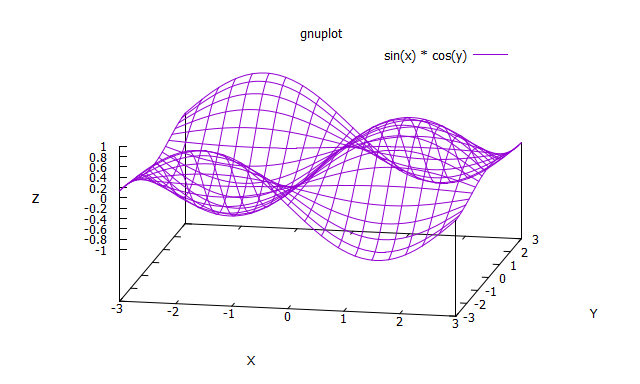
\includegraphics[width=1\textwidth]{figuras/cap_3/secao_3/gnuplot_sincos.png}
\caption{Gráfico gerado utilizando o gnuplot para a função $sin(x) . cos(y)$}
\label{gnu_sincos}
\end{figure}

\begin{figure}[htp!]
\centering
\lstinputlisting[language=gnuplot]{codigos/gnuplot.gnu}
\caption{Script utilizado para a geração do gráfico da figura \ref{gnu_sincos}}
\label{gnu_sincos_code}
\end{figure}

Dentro do contexto do trabalho, a utilização da ferramenta auxilia na geração de gráficos contendo os resultados dos testes, feitos por meio do simulador the ONE, e da análise dos resultados apresentados por meio de gráficos.

\section{Conclusão do Capítulo}\label{sec:conclusao_cap_3}

A primeira seção deste capítulo apresentou um breve resumo sobre o simulador the ONE, incluindo explanações sobre os protocolos implementados, arquitetura simplificada e funcionamento básico. Tal simulador é muito importante para o desenvolvimento da técnica objetivada, visto as facilidades oferecidas e o seu desempenho.

A linguagem Java, apresentada de forma sucinta na seção \ref{sec:java}, é de grande valia para a implementação da técnica, visto as abstrações oferecidas e a linguagem utilizada para o desenvolvimento do simulador.

A análise dos resultados da técnica é facilitada por meio dos relatórios gerados pelo simulador The ONE e da ferramenta gnuplot, apresentados nas seções \ref{sec:theONE} e \ref{sec:gnuplot}, respectivamente.

As ferramentas utilizadas são de grande importância para o projeto, contribuindo de forma significativa na construção da base necessária para o desenvolvimento e análise da técnica. Além disso, o estudo das ferramentas proporciona melhor entendimento e interação com assuntos relacionados às áreas de \emph{Simulação de Ambientes} e \emph{Probabilidade e Estatística}, permitindo adquirir conhecimentos não vistos durante o curso de Ciência da Computação.

